\documentclass[tikz,border=6pt]{standalone}
\usetikzlibrary{arrows.meta,positioning}
\begin{document}
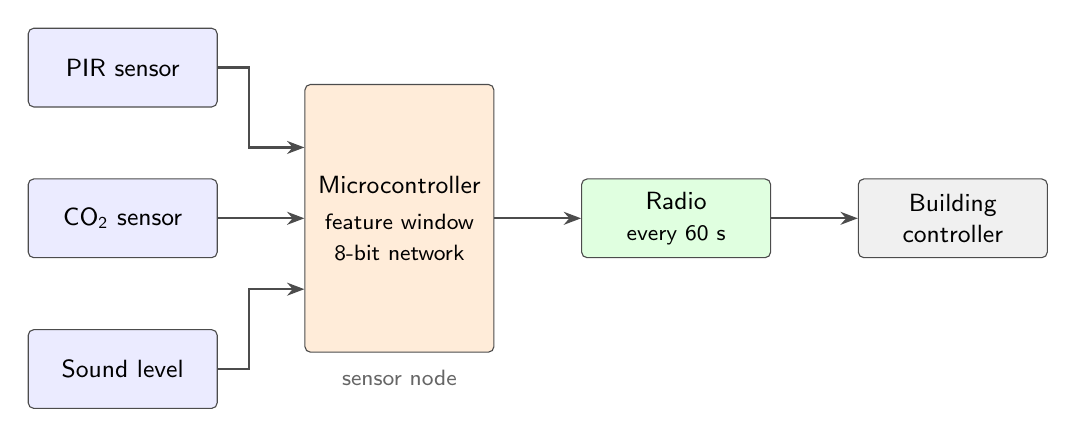
\begin{tikzpicture}[font=\sffamily\small, node distance=9mm and 11mm,
  box/.style={draw=black!70, rounded corners=2pt, minimum width=24mm, minimum height=10mm, align=center, fill=#1},
  box/.default={blue!8}, arr/.style={-{Stealth[length=2.2mm]}, thick, black!70}]
  \node[box] (pir) {PIR sensor};
  \node[box, below=of pir] (co2) {CO\textsubscript{2} sensor};
  \node[box, below=of co2] (mic) {Sound level};
  \node[box=orange!15, right=of co2, minimum height=34mm] (mcu) {Microcontroller\\[2pt]\footnotesize feature window\\\footnotesize 8-bit network};
  \node[box=green!12, right=of mcu] (radio) {Radio\\\footnotesize every 60 s};
  \node[box=gray!12, right=of radio] (bms) {Building\\controller};
  \draw[arr] (pir.east) -- ++(4mm,0) |- ([yshift=9mm]mcu.west);
  \draw[arr] (co2) -- (mcu);
  \draw[arr] (mic.east) -- ++(4mm,0) |- ([yshift=-9mm]mcu.west);
  \draw[arr] (mcu) -- (radio);
  \draw[arr] (radio) -- (bms);
  \node[below=1mm of mcu, font=\sffamily\footnotesize, black!60] {sensor node};
\end{tikzpicture}
\end{document}
